\documentclass[twocolumn]{article}
\usepackage[margin=0.6in,columnsep=0.15in]{geometry}
\usepackage[utf8]{inputenc}
\usepackage{stix}
\usepackage{microtype}
\usepackage[usenames,dvipsnames]{xcolor}
\usepackage[colorlinks,citecolor=Gray,urlcolor=Gray,linkcolor=Cyan]{hyperref}
\usepackage[tiny]{titlesec}

\usepackage{authblk}
\renewcommand\Affilfont{\itshape\small} % chktex 6

\usepackage[normal]{caption}
\DeclareCaptionLabelSeparator{pipe}{ $|$ }
\captionsetup{labelsep=pipe}
\renewcommand{\captionfont}{\small}
\renewcommand{\captionlabelfont}{\bfseries}

\usepackage[sort&compress]{natbib}
\bibliographystyle{abbrvnat}
\renewcommand\cite{\citep}
\usepackage{doi}

\usepackage{graphicx}
\usepackage{mathtools}
\usepackage{booktabs}
\usepackage{tabularx}
\usepackage{tikz}

\usepackage[export]{adjustbox}

\title{The range of semi-local density functionals in van der Waals systems: Supplementary information}

\author[1]{Jan Hermann}
\author[1]{Matthias Scheffler}
\author[2,*]{Alexandre Tkatchenko}
\affil[1]{Fritz-Haber-Institut der Max-Planck-Gesellschaft, Faradayweg 4--6, 14195 Berlin, Germany}
\affil[2]{Physics and Materials Science Research Unit, University of Luxembourg, 162A Avenue de la Faïencerie, L-1511 Luxembourg}

\date{}

\setcounter{secnumdepth}{0}

\begin{document}

\nocite{achemso-control}

\maketitle

\begingroup
\renewcommand\thefootnote{}\footnote{$^*$Email: alexandre.tkatchenko@uni.lu}%
\addtocounter{footnote}{-1}%
\endgroup

\section{Computational details}

All resources for the manuscript, including the manuscript itself, can be found in a Git repository~\cite{GitRepo} and related data files~\cite{DataH5,DataCaf}.
This includes scripts used to generate input files, all inputs and output files, data processing scripts, data, figures, and \LaTeX\ source files.
Here, we give a summary of the computational protocol.

All DFT calculations were done with FHI-aims~\cite{BlumCPC09}, which uses atom-centered basis sets with numerical radial parts.
We used the \texttt{tight} default basis set and grid settings, which ensure numerical convergence to 0.1\,kcal/mol in binding energies for van der Waals (vdW) systems.

\begin{figure*}
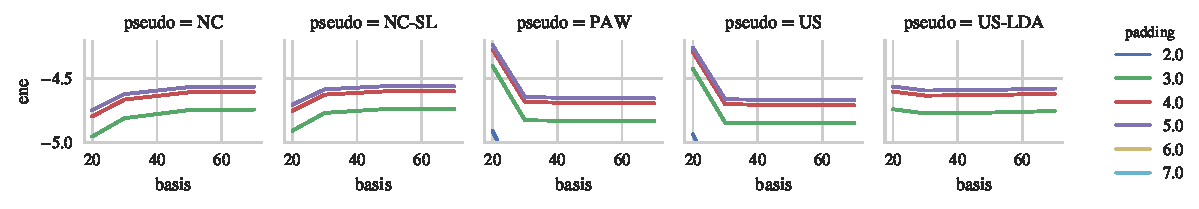
\includegraphics[center]{../media/bz-tests-padding-basis}
\caption{\textbf{Label.}
Text.
}\label{fig:bz-tests-padding-basis}
\end{figure*}

The VV10 nonlocal functional was evaluated with Quantum Espresso~\cite{GiannozziJPCM09}, which uses plane-wave basis sets, and so is restricted to periodic boundary conditions only.
To calculate isolated molecular systems, we used norm-conserving Vanderbilt pseudopotentials~\cite{HamannPRB13}, the plane-wave cutoff of 30\,Ry, and separated the periodic images with 8\,\AA\ of vacuum, which converges vdW binding energies to 0.1\,kcal/mol (Figure~\ref{fig:bz-tests-padding-basis}).

For crystals, $k$-point grids with density of at least 0.8\,\AA\ in reciprocal space were used for all DFT, MBD, and VV10 calculations.

Both VV10 and MBD depend on the electron density, and in principle should be calculated for each density functional separately, but in practice the differences between the densities from different functionals are of the sort that changes the vdW energies only negligibly.
Therefore, we calculated MBD on PBE densities, and VV10 on the originally suggested combination of reparameterized PW86 exchange and PBE correlation.

All molecular crystal geometries were taken directly from the respective benchmark sets without any relaxation, and can be found in the repository~\cite{GitRepo} or as supplementary data.

\section{Supplementary results}

\begin{figure*}
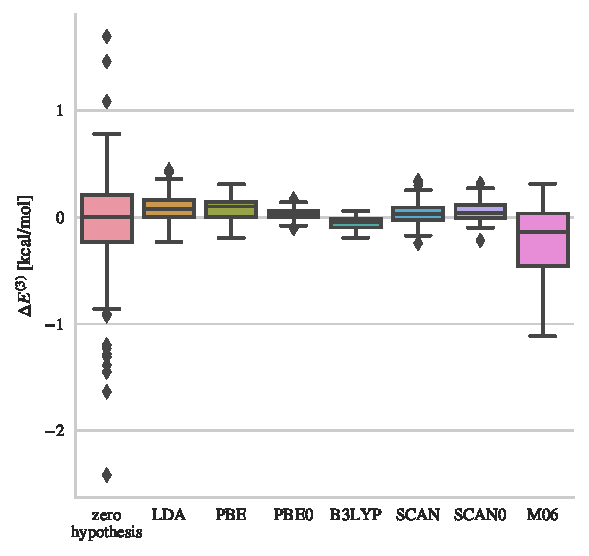
\includegraphics[center]{../media/3-body}

\caption{\textbf{Distributions of relative errors in 3-body interaction energies on the 3B-69 set.}
The box-and-whisker plot is of the same kind as Figure 1 in the main text.
The ``zero hypothesis'' corresponds to a method which always gives zero 3-body interaction energy.
}\label{fig:3-body}
\end{figure*}

\begin{figure*}
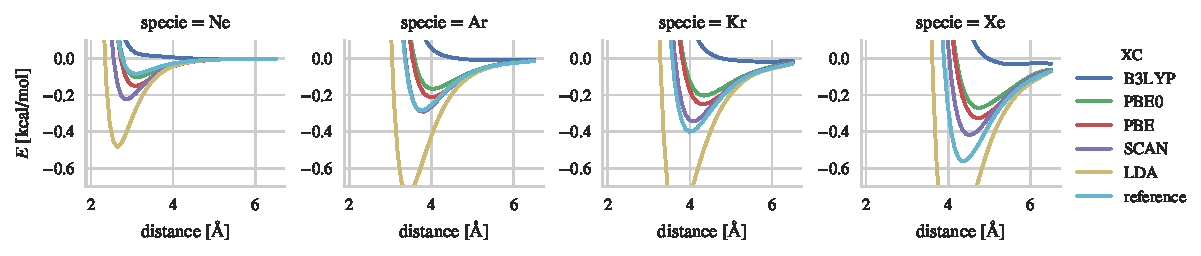
\includegraphics[center]{../media/mbd-rare-gas}
\caption{\textbf{Binding curves of rare-gas dimers.}
The reference is a highly accurate empirical potential parametrized on experimental data.
}\label{fig:mbd-rare-gas}
\end{figure*}

Figure~\ref{fig:3-body} shows the errors of density functionals in 3-body interaction energies calculated on the 3B-69 set~\cite{RezacJCTC15}.
Figure~\ref{fig:mbd-rare-gas} shows the interaction curves of rare-gas dimers calculated with different density functionals.

\begingroup
\renewcommand{\section}[2]{}
\setlength\bibsep{0pt}
\footnotesize
\bibliography{refs-zotero,refs}
\endgroup

\end{document}
